\section{Analyse du mode de gestion}

\begin{frame}
    \tiny
    \frametitle{Analyse du mode de gestion}

    \begin{columns}
        \column{0.66\textwidth}
        La visualisation ci-contre présente la répartition des modes de gestion pour les CA du mois :

        \begin{itemize}
            \item \textbf{<< part_ca_mode_non_permanent|number >>\%} des achats sont réalisés en \textbf{non permanent}
            \item \textbf{<< part_ca_mode_permanent|number >>\%} des achats sont réalisés en \textbf{permanent}
        \end{itemize}

        \column{0.33\textwidth}
        \centering

        \begin{figure}
            \centering
            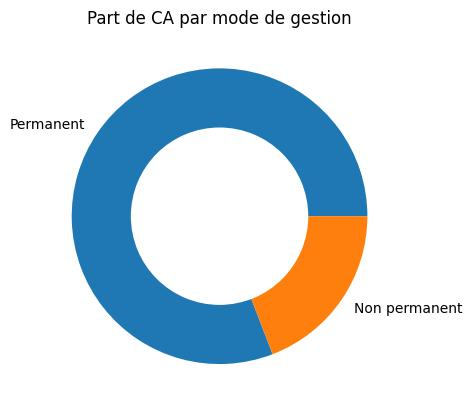
\includegraphics[width=1\textwidth]{assets/__ca_total_par_mode_de_gestion}
        \end{figure}
    \end{columns}

    \begin{figure}[h]
        \centering
        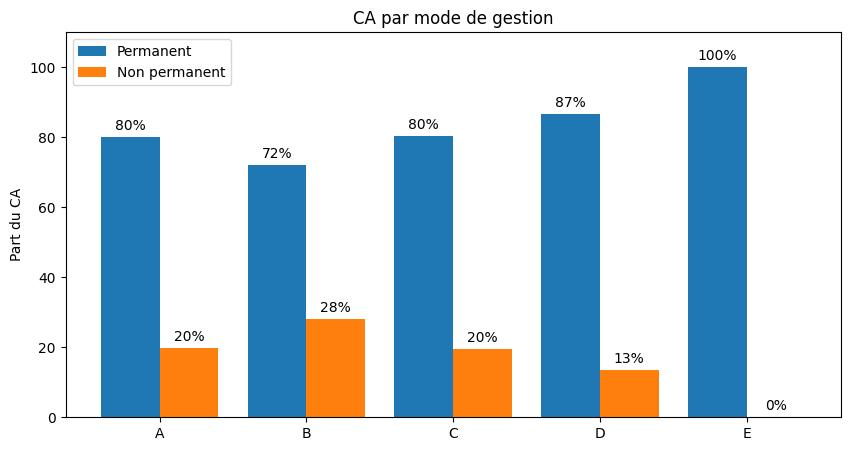
\includegraphics[height=3cm]{assets/__ca_magasins_par_mode_de_gestion}
    \end{figure}

    D’après ces visualisations, \textbf{<< magasins_permanents_seulement|length >>}
    << pluralize(
        magasins_permanents_seulement|length,
        'point de vente a commandé',
        'points de vente ont commandé',
    ) >>
    \textbf{uniquement en PERMANENT.}
\end{frame}
